\documentclass[12pt,a4paper]{report}
\usepackage{fbe_tez_with_history}
\usepackage{enumerate}
\usepackage{enumitem}
\usepackage[utf8]{inputenc}
\usepackage{graphicx}
\usepackage{float}
\usepackage{hyperref}
\usepackage{subfig}
\usepackage{mathtools}
\graphicspath{ {images/} }
\title{Evaluation of Movie Recommendation Algorithms}

\date{\emph{03.01.2019} \\ \emph{Version 1.0} }

\author{CmpE 492 Senior Project\\
By: Abdurrahim Eskin and İsmail Levent Baş \\
Advisor: Prof. Fikret S. Gürgen \\
}

\begin{document}
\pagenumbering{roman}

\maketitle

% VERSION HISTORY
\begin{history}

\begin{table}[htp]
\begin{center}
\begin{tabular}{|c|c|p{10cm}|}
\hline
\textbf{Version} & \textbf{Date} & \textbf{Explanation} \\
\hline
0.0 & 27.09.2018 & Initial draft of problem definition and the document template \\
\hline
0.1 & 02.10.2018 & Introduction and constraints sections are added \& previous draft's errors are fixed \\
\hline
0.2 & 03.10.2018 & Problem statement section is added and constraints section is rewritten \\
\hline
0.3 & 15.10.2018 & Background and Method sections are added \& fixed previous draft's errors \\
\hline
0.4 & 21.10.2018 & Improved Method section \& added formulas \\ \hline
0.5 & 31.10.2018 & Fixed previous draft's errors \& added Conclusions and Future Work  \\
\hline
0.6 & 05.11.2018 & Added new algorithm in Method section  \\
\hline
0.7 & 14.11.2018 & Fixed previous draft's errors \& improved Method section \\
\hline
0.8 & 01.12.2018 & Changed Introduction section \& code sample is added \\
\hline
0.9 & 15.12.2018 & Improved Background section \& added new formulas to Method section  \\
\hline
1.0 & 29.12.2018 & Evaluation section is added \& improved the Conclusions and Future Work section \\
\hline
\end{tabular}
\end{center}
\end{table}

%\clearpage %to prevent LaTeX from placing the following table at the center of the page

\end{history}

\begin{abstract}
Recommendation systems are gaining importance, especially with the development of new technologies and advanced machine learning algorithms. However, in the of case recommending items to users we have to be very careful about which dimensions to consider. We have to consider the domain of recommendation and also the purpose of the recommendation. Moreover, we have to come up with the best system, given the data we have, that is good at recommending items to the users. In our study, we will be building up a movie recommendation system that is evaluated using certain metrics such as MAE, MSE and RMSE. We will be closely interested in the performance of such a recommender system as we apply certain algorithms. The algorithms that we will be applying are User-User Collaborative Filtering, Item-Item Collaborative Filtering and Singular Value Decomposition.
\end{abstract}

\tableofcontents

\chapter{Introduction}

\pagenumbering{arabic}

With the increasing importance of Web in our lives as a medium for consumption, millions of people have left their trace on the Internet; when they buy a product, rate a movie or book, use a search engine, listen to a song or up-vote a post in a blog. Hence, the ease of use of Web has enabled users to provide both explicit and implicit feedback for other users even if they are not aware of this fact, giving rise to the need of a system to make use of this abundance of feedback data. The system, based on that data, can recommend movies, songs, products and even people to other users. Evidently, this system is a recommendation system. 

In this project, we will be examining certain recommendation algorithms for movies. We will test the recommendation system itself and evaluate the performance of the underlying algorithms by using metrics such as Mean Square Error (MSE), Precision@n, Recall and Mean Absolute Error (MAE). In Section 2.2, we will give background information about some types of recommendation algorithms. As we implement these recommendation algorithms we will use a dataset that was collected and made available by GroupLens Research from the movie recommendation service MovieLens. This dataset will be explained further in Section 2.3. Then in Section 3, we will explain our method in detail and discuss implementations of various algorithms using Python programming language. In Section 4, we will be sharing the evaluation results of recommendation algorithms.
  
 
\section{Problem Statement and Constraints}

The aim of this project is to find the most accurate recommendation algorithms to be used in a recommendation system. What we mean by accurate is that we want to be able to come up with implementations of algorithms that are best at predicting top-N recommendations to a certain user or what rating that user will give to the movie that he or she hasn't seen yet. We would like to know if we can determine the accuracy of this prediction by inspecting metrics related to the recommendation system. 

Even though what we want to accomplish is very clear, the road to the solution of our problem deemed to be more complex than we thought in the first place. Since we are dealing with users, items and ratings of items given by the users, there is a lot of data to be processed. We are aware of the fact that, eventually, we may have to use Big Data solutions such as Spark, Hadoop and etc. 

\chapter{Background} 

\section{Overview of Recommendation Systems}

Recommendation systems have become very popular in many domains such as e-commercial services like Amazon.com, movie database website IMDB and streaming services like Netflix. When we talk about domain of recommendation, what we really want to know is, what's being recommended. Are we recommending news articles? Are we recommending products? Are we recommending bundles, where instead of a particular product, we're interested in knowing  whether the customer is likely to buy product x, y and z together. 

Are we recommending sequences, like a music playlist, where it may not just be the set of songs, but that the
order of those songs may matter. And a particularly interesting property of a recommendation domain is the way in which we treat
items that have already been experienced.

In some domains, we may be primarily interested in recommending new items, things the users haven’t experienced yet. If the users come looking for a movie, most of the time, they are looking to see a movie that they haven't seen or read a book that they haven't read. In other domains, most of the things that are being recommended are products users have experienced before. In Spotify, which is a music streaming service, the recommendation system is most likely to recommend which song to play next, where 90\% of the music the users listen to is the music they have heard before. With groceries, the system may recommend what to buy without limiting to things the users have never eaten, since people buy the same groceries again and again. 

If we consider another domain such as search engines, what they are doing is actually recommending web pages to the user. We don't always think of a search engine as a recommendation system. But indeed in Google's case, we give it a search phrase or a set of terms and the engine comes back with the suggested (recommended) pages it thinks we would like.

Another aspect to consider before developing a recommendation system, is the purpose of the recommendation. In many cases the purpose is simple, the recommendation is almost an end in itself,
we want the customers to buy or consume or otherwise
take up the recommendation we give them.
If it's music, we want them to listen to it, if it's a movie, we want them to go watch it. But in other cases the recommendations are aggregated as a form of education, or as a form of building community. And understanding whether recommendations are part of a larger purpose which helps us build the system in a way tailored to the user's needs.

Another dimension to consider in recommendation systems is the dimension of context. What are the users doing at the time of the
recommendation? Are they shopping? Are they listening to music Are they hanging out with other people? And how does that constrain the recommending system? If the users are listening to music, for instance, the last thing they want is for the end of every song to have a dialogue box pop up recommending which song the system thinks they would like next.

While listening, the users may want to change the song and that may change the recommendation the system has made. If the system predicts the user is mostly risk
averse, it'll just play music. It has a good reason to believe the user will like. If it thinks the user may be into new experiences, it might mix in more riskier and unfamiliar music. Moreover, if the system knows that the user is hanging out with other people, it may make a recommendation for groups rather than for individuals. Obviously, all of these things can affect the level of attention or the degree to which the user is willing to accept an interruption.

Next dimension that we should consider is the data that the recommendation system is based on. Recommender systems, in the broad sense, are based on somebody's opinion, sometimes only the user that the system is recommending items to, but more often some other people's as well. One of the things we look at is whose opinion is the recommender based on. Is it experts? Is it everybody? Is it just people like the user herself? We need to answer these kinds of questions before diving into the world of recommending items to users and for this project this is, indeed, what we have done.

\section{Recommendation Algorithms}

\subsection{Non-Personalized Recommendation}

 A lot of recommendations and a lot of the way we think about recommendation is personalized, such as Netflix suggesting what we might want to watch next. But there's a variety of situations in which non-personalized recommendation is still very useful. One case is when there are new users, where we know very little about the new user. We can't personalize, but we still want to be able to provide recommendations that the user may find useful and actionable. It is non-personalized because it is the same recommendation to every user and not specific to each user. Non-personalized recommendations can be very efficient to compute (such as how many people bought this item) and they are easy to understand. These recommendations are normally concerned with the popularity of the item (top rated shows, charts of songs etc.)
 
 \subsection{Content-based Recommendation}
 
In recommendation systems, content is a set of attributes or a set of descriptors that describe the things that we're
recommending to the users. For instance, in the case of movies content might include actors, directors or genres. We can also think of more complex products, including services in a hotel which might be a 24 hours available staff, room servies or a pool. Those may be the attributes that could lead to recommending a particular hotel for the user.

Hence, the key idea of a content-based recommendation system is the fact that we model items according to relevant attributes which by itself usually takes some human effort. Then we model and learn user preferences structured by those same attributes. Moreover, we can infer a profile from user actions. For instance, as somebody buys something, reads it, or clicks on it, we can figure out what all of the descriptive keywords or the attributes for that item that they have just expressed a preference about implicitly. If the user chooses to read an article about technology, we can aggregate all the relevant keywords, tags etc. about the article to build a profile. We can do the same thing with explicit user ratings. In either case, we're really talking about taking a vector of user ratings and processing that against a database of content attributes to build a content profile.
In fact what many systems do is to merge the two together.
They take explicit and implicit ratings and merge those
into a comprehensive set of information about user interactions and preferences and from that they infer keyword and attribute
preferences to build a profile. After creating the profile the system can recommend new items to the user.

\subsection{Dimensionality Reduction Recommendation}

The motivation behind dimensionality reduction, is that a ratings matrix, is a highly over fit representation of user tastes and item descriptions which means that we end up matching things to individual details, rather than, to underlying preferences and tastes. If we could represent user tastes and preferences in a much more compact and portable way, we can build a simple recommendation system for that specific preference. By using SVD (Singular Value Decomposition) algorithm, we can take the rating matrix and compress it into a smaller, compact, well-robust matrix that has as little loss as possible and in the process of smoothing out the matrix, we might smooth over little attributes and artifacts. By doing that, we would be compressing the ratings matrix into a smaller taste space and recommending new items using that compressed ratings matrix.


\subsection{Nearest Neighbor Collaborative Filtering}

In collaborative filtering, we ignore the user and item attributes. We don't care what's in the item and we don't care who the user is. We only look at the interactions between users and items. And we mine patterns from these, such as looking at what users similar to a certain user also bought. Collaborative filtering allows us to develop algorithms that operate independently of the characteristics of the particular items being recommended. Nearest neighbor collaborative filtering algorithm is basically a collaborative filtering algorithm that is combined with k-nearest neighbor algorithm. Nearest neighbor part of the algorithm selects the set of neighbors that are close (similar) to the user or the item that we are predicting a rating for. There are two types of collaborative filtering algorithms:

1.User-User Collaborative Filtering: When we want to recommend an item to a user, we scan every neighbor of that user and see what those neighbors have rated that certain item. We use this knowledge to come up with a prediction of rating of that item before we recommend it to the user.

2.Item-Item Collaborative Filtering: In item-item collaborative filtering we are interested in knowing how much similar an item that we want to predict the rating for is to the other items that the user has rated before. This similarity has nothing to do with the item's attributes. Instead, what similarity means is that how other users treat the compared items the same in terms of like and dislike.


\section{MovieLens Dataset}

In this project, we will be using a dataset called MovieLens 100K Dataset from GroupLens Research. This dataset was collected from a movie recommendation system called MovieLens.

This dataset consists of:
\vspace{-5mm}
\begin{itemize}
    \item 100,000 ratings (1-5) from 943 users on 1682 movies.
    \item Users that have rated at least 20 movies. 
    \item Simple demographic information for the users (age, gender, occupation, zip)
\end{itemize}
 Below, a part of rating, user and movie tables from the dataset can be found:
 \begin{figure}[h]%
    \centering
    \subfloat{{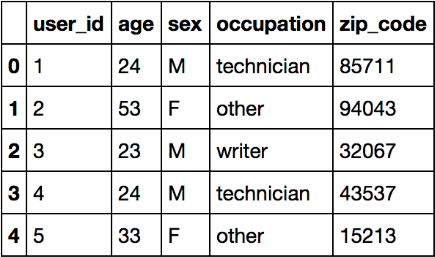
\includegraphics[width=5cm]{user.png} }}%
    \qquad
    \subfloat{{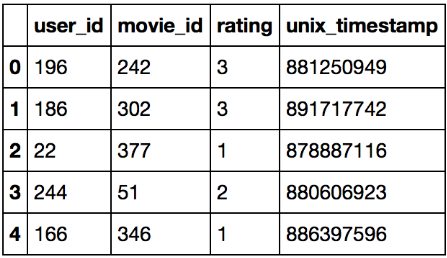
\includegraphics[width=5cm]{rating.png} }}%
    \caption{User and rating tables.}%
    \label{fig:example}%
\end{figure} 

 \begin{figure}[h]
    \centering
    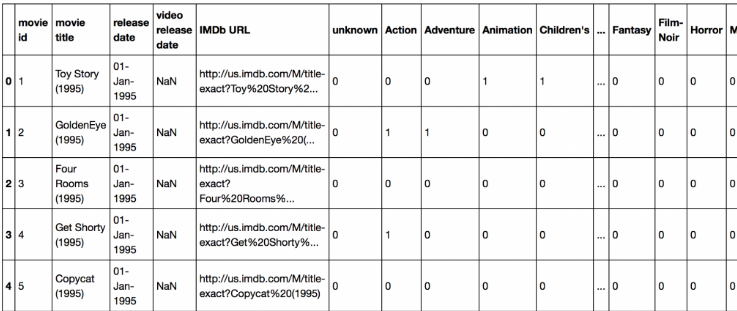
\includegraphics[width=14cm, height=6cm]{movie.png}
    \caption{Movie table.}
\end{figure}


\chapter{Method}
\section{User-User Collaborative Filtering Method}

Firstly, we want to define the scoring function as s(u,i) which is used to calculate the predicted rating of item i by user u. We compute the s(u,i) as follows:
\vspace{-5mm}
\begin{enumerate}
    \item For all the users v $\neq$ u, we compute $w_{u,v}$ which is a similarity metric (e.g. cosine similarity) that is used to measure the similarity between users u and v. In this project we will be using Pearson correlation as our similarity metric:
    $$w_{u,v} = \sum_{i\in I} \frac{(r_{u,i}-\overline{r_u})(r_{v,i}-\overline{r_v})}
    {\sigma_u\sigma_v}$$
    In the above formula, $r_{u,i}$ is the rating of item i that is given by user u and I is the set of all items in the system.
    \item We select a neighborhood of users V $\subset$ U, where U is a set of all users in the system and V is the selected neighborhood.
    \item We compute the prediction:
    $$s(u,i) = \overline{r_u} +
    \frac{\sum_{v \in V}(r_{v,i}-\overline{r_v})w_{u,v}}
    {\sum_{v \in V}w_{u,v}} $$
\end{enumerate}

\section{Item-Item Collaborative Filtering Method}
In order to find the predicted ratings same steps can be used as used in user-user collaborative filtering. However, here, we want to compute the similarity between items not users. Similarity between item i and item j can be computed as follows:
$$w_{i,j} = \frac{\sum_{u \in U} (r_{u,i}-\overline{r_i})(r_{u,j}-\overline{r_j}) }{\sqrt{\sum_{u \in U}(r_{u,i}-\overline{r_i})^2}
\sqrt{\sum_{u \in U}(r_{u,j}-\overline{r_j})^2}}$$

We compute the prediction for item-item collaborative filtering as follows:
$$s(u,i) = \overline{r_i} + \frac{\sum_{j \in N(i,u)} w_{i,j} (r_{u,j}-\overline{r_j})}{\sum_{j \in N(i,u)}|w_{i,j}|}$$
In the above formula, N(i,u) is the set of k most similar items to i that user u has rated.

Below, a code snippet from our project can be seen:

\begin{figure}[h]
    \centering
    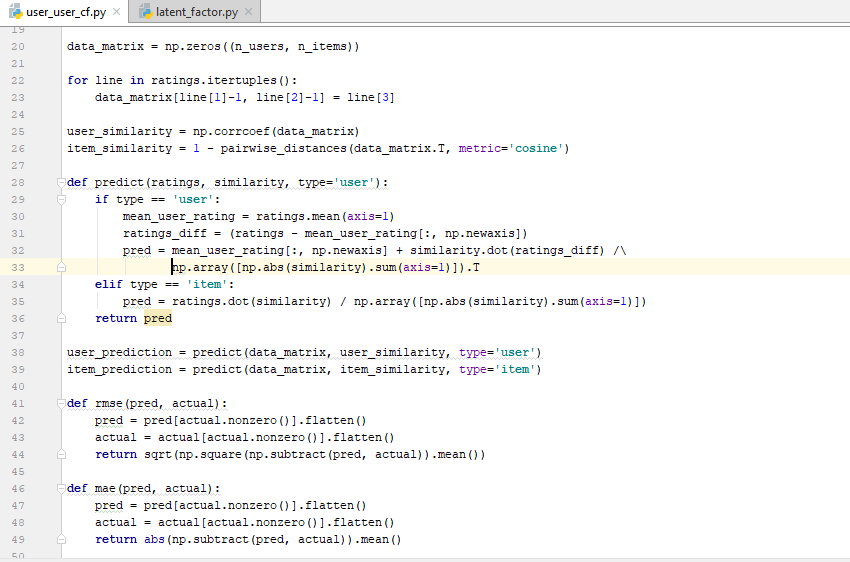
\includegraphics[width=15cm, height=10cm]{code.png}
    \caption{Code snippet in Python.}
\end{figure}

\section{Singular Value Decomposition (SVD) Method}

We want to compute SVD of our ratings matrix R where the rating of user u for item i will be denoted by $ r_{u,i} $ as follows:

\begin{figure}[H]
    \centering
    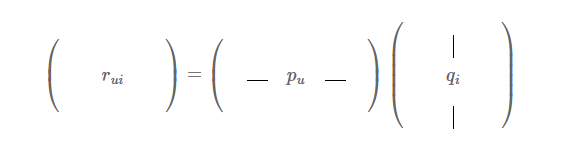
\includegraphics[width=10cm, height=3cm]{svd.png}
\end{figure}

 The value of $r_{u,i}$ is the result of a dot product between two vectors: a vector $p_u$ which is specific to the user u, and a vector $q_i$ which is specific to the item i:
  $$r_{u,i}=p_u.q_i$$
   where '.' stands for the usual dot product.
   Finding such vectors $p_u$ and $q_i$ for all users and items can be done by solving the following optimization problem:
  $$ \min_{p_u, q_i\\p_u \perp p_v\\ q_i \perp q_j}\sum_{r_{ui} \in R} (r_{ui} - p_u \cdot q_i)^2 $$
  
  We will use SGD (Stochastic Gradient Descent) to find a solution to this optimization problem. Once all the vectors $p_u$ and $q_i$ have been computed, we can estimate all the ratings we want using the dot product of these two matrices.
  

\chapter{Evaluation}

After applying the algorithms defined in Method section, we carefully evaluate our algorithms using some metrics that are popularly used in many recommendation systems.

These evaluation metrics are as follows: 
\vspace{-5mm}
\begin{itemize}
    \item Mean Absolute Error (MAE): A widely used predictive accuracy metric is the mean absolute error, or MAE. Mean absolute error takes the sum of the absolute value of difference between the user’s rating and the predicted rating and divides it by the number of items considered.
    \item Mean Squared Error (MSE):  Mean squared error takes the sum of the squared difference between the user’s rating and the predicted rating and divides it by the number of items considered.
    \item Root Mean Square Error (RMSE): Root mean square error simply takes the square root of the mean squared error (MSE).
    \item Precision@N: Precision@N is the proportion of recommended items in the top-N set that are relevant.
    \item Recall@N: Recall@N is the proportion of relevant items found in the top-N recommendations.
\end{itemize}

After considering these metrics above, we have evaluated our recommendation system and the evaluation results can be seen below:

\begin{table}[htp]
\begin{center}
\begin{tabular}{|p{5cm}|c|c|c|c|c|}
\hline
\textbf{Evaluation Metrics} & \textbf{MAE} & \textbf{MSE} & \textbf{RMSE} & \textbf{P@N} & \textbf{R@N} \\
\hline
User-User CF & 2.4238 & 7.0638 & 2.6577 & 0.65 & 0.17 \\
\hline
Item-Item CF & 2.7061 & 8.7036 & 2.9501 & 0.55 & 0.14 \\
\hline
SVD & 3.5421 & 15.664 & 3.9577 & 0.46 & 0.11 \\
\hline
\end{tabular}
\end{center}
\end{table}


{ \chapter{Conclusions and Future Work}}

Evaluating movie recommendation algorithms is not a simple job, thus, we are far from finished. So far, we have done enough research to understand how several recommendation algorithms work and have written enough code in Python language to understand how certain recommendation algorithms are evaluated based on different evaluation metrics. In future, we will be examining more recommendation algorithms besides collaborative filtering and dimensionality reduction algorithms. We will consider using a bigger dataset than the one we have used while applying our algorithms. Spark seems to be the ideal choice when dealing with such a big dataset (e.g. MovieLens 1M dataset), hence, we will use our time wisely to understand the ways of using Spark in our recommendation system as it is more likely to enhance the performance of the system. We may also consider other evaluation metrics besides precision, recall and other error metrics (e.g. MAE).

\begin{thebibliography}{}

\bibitem{linden}
Linden, G., Smith, B., and York, J. (2003). Amazon.com recommendations: Item-to-item collaborative filtering. 

\bibitem{waila}
Waila, P., Singh, V., Singh, M. (2016). A Scientometric Analysis of Research in Recommender Systems.

\bibitem{ricci}
Ricci, F., Rokach, L., Shapira, B., and Kantor, P.B. (2011). Introduction to Recommender Systems Handbook.

\bibitem{book}
Aggarval, Charu C. (2016). Recommender Systems, The Textbook.

\bibitem{claypool}
Claypool M, Gokhale A, Miranda T, Murnikov P, Netes D, Sartin M.(1999). Combining content- based and collaborative filters in an online newspaper.

\bibitem{basu}
Basu C, Hirsh H, Cohen W.(1998). Recommendation as classification: using social and content-based information in recommendation.

\bibitem{schwab}
Schwab I, Kobsa A, Koychev I.(2001). Learning user interests through positive examples using content analysis and collaborative filtering.

\bibitem{sarwar}
Sarwar B, Karypis G, Konstan J, Reidl J. Item-based collaborative filtering recommendation algorithms

\end{thebibliography}


\end{document}
